\begin{homeworkProblem}
The \textit{finite difference time domain (FDTD)} is a widely used tool in electromagnetics \cite{taflove}. The FDTD method solves Maxwell's equations using discrete derivative operators. In the same way FDTD method can be applied to solve Schr\"odinger equation. The numerical scheme used to solve the Schr\"odinger equation differs from the scheme found in electromagnetics. In this project, a simple discretization of the one-dimensional Schr\"odinger's equation is presented and numerical results are compared with theoretical calculations. 

The FDTD technique simulates the time revolution of the wave function in the space where the potential could be any arbitrary function. The stability of time-marching FDTD scheme is analyzed and a bound for the time step is given. The maximum bound step is a bound which avoids the accumulation of the numerical errors \cite{antonio004}.

 In practical calculations, because of the finite capacity of the memories, the area of computation must be limited to appropriate size.  When the natural domain for the problem being solved is infinite the use of absorbing (transparent) boundary conditions are necessitated to eliminate undesirable spurious reflections at boundaries \cite{shibata,kosloff}. 

In the successive sections first the discrete version of the Schr\"odinger's equation is given and then the theoretical and numerical evolution of a normalized one-dimensional wave packet is presented. Stability analysis and approximate artificial boundary conditions and the corresponding update equations are given afterwards. 
\begin{homeworkSection}{FDTD Calculation of 1D Schr\"odinger Equation}
One dimensional Schr\"odinger equation for a real potential is:
\begin{equation}
i\hbar\pd{\Psi(z,t)}{t}=-\frac{\hbar^2}{2m}\pdt{\Psi(z,t)}{z}+V(z)\Psi(z,t)
\end{equation}
Assume that we decompose the wave function to its real and imaginary parts as:
$$\Psi(z,t)=\Psi_r(z,t)+i\Psi_i(z,t)$$
then:
\begin{align}
-\hbar\pd{\Psi_i(z,t)}{t}&=-\frac{\hbar^2}{2m}\pdt{\Psi_r(z,t)}{z}+V(z)\Psi_r(z,t)\label{P5-real}\\
\hbar\pd{\Psi_r(z,t)}{t}&=-\frac{\hbar^2}{2m}\pdt{\Psi_i(z,t)}{z}+V(z)\Psi_i(z,t)\label{P5-imag}
\end{align}

Two couple partial differential equations can be numerically analyzed using FDTD method. If we discretize the space and time as $z=s\Delta z$ and $t=n\Delta t$ and using central difference scheme for the ordinary spatial nodes the desired update equations can be obtained.  In order to set up two implementable update equations we have to calculate $\Psi_r$ at integer values of $n$ while $\Psi_i$ are calculated at the half-integer values of $n$. The discredited version of the equation \eqref{P5-real} at $t=n\Delta t$ and $z=s\Delta z$ is given below. For convenience we use $\Psi(s,n)$ instead of $\Psi(s\Delta z,n\Delta t)$ in the rest of this report:
\begin{equation}\label{P5-1}
\hbar\frac{\Psi_i(s,n+0.5)-\Psi_i(s,n-0.5)}{\Delta t}=
\frac{\hbar^2}{2m}\frac{\Psi_r(s+1,n)-2\Psi_r(s,n)+\Psi_r(s,n-1)}{(\Delta z)^2}-V(s\Delta z)\Psi_r(s,n)
\end{equation}  
Discretization of the equation \eqref{P5-imag} at $t=(n+0.5)\Delta t$ and  $z=s\Delta z$ leads to the following equation:
\begin{multline}\label{P5-2}
\hbar\frac{\Psi_r(s,n+1)-\Psi_r(s,n)}{\Delta t}=\\
-\frac{\hbar^2}{2m}\frac{\Psi_i(s+1,n+0.5)-2\Psi_i(s,n+0.5)+\Psi_i(s-1,n+0.5)}{(\Delta z)^2}+V(s\Delta z)\Psi_i(s,n+0.5)
\end{multline}

The equations \eqref{P5-1} and \eqref{P5-2} can be rewritten in a more convenient form:
\begin{equation}\label{coupled1}
\Psi_i(s,n+0.5)=\Psi_i(s,n-0.5)+\xi\left[\Psi_r(s+1,n)-2\Psi_r(s,n)+\Psi_r(s,n)\right]-\frac{\Delta t V(s\Delta z)}{\hbar}\Psi_r(s,n)
\end{equation}


\begin{equation}\label{coupled2}
\Psi_r(s,n+1)=\Psi_r(s,n)-\xi\left[\Psi_i(s+1,n+0.5)-2\Psi_i(s,n+0.5)+\Psi_i(s,n+0.5)\right]+\frac{\Delta t V(s\Delta z)}{\hbar}\Psi_i(s,n)
\end{equation}
        
        
In above equations $\xi$ is defined as:
$$\xi=\frac{\hbar\Delta t}{2m(\Delta x)^2}$$
\end{homeworkSection}

In this project Drichlet boundary condition for initial wave function is chosen. It's assumed that the wave function is a Gaussian wave packet at $t=0$ this wave function evolves in the light of Schr\"odinger's equation. The initial normalized wave function is:
\begin{equation}
\Psi(z,t=0)=\left({\frac{2}{\pi\sigma^{2}}\right)^{\frac{1}{4}}\exp\left(\frac{-(z-z_0)^2}{\sigma^2}\right)\exp\left(\frac{2\pi i(z-z_0)}{\lambda_e}\right)
\end{equation}

wherein $z_0$ is electron's initial position . we choose $z_0=0$ in our simulations. $\lambda_e$ is the electron de Broglie's wave length. We choose $\Delta z=0.1 \mathrm{nm}$ , $\Delta t=0.02 \mathrm{fs}$ , $\sigma=\lambda_e=5\mathrm{nm}$. In our computer program we use $\mathrm{nm}$  and $\mathrm{fs}$ as the unites of length and time respectively. The mass of electron is expressed in the term of $\mathrm{em}$. Electron's rest mass is $0.511 \mathrm{Mev}$ . In this case reduced Planck's constant is $\hbar\approx 0.658 \mathrm{eV.fs}$.  
This wave packet propagates in the free space ($V=0$) . 


\end{homeworkSection}
%-----------------------------------------------------------------------------------
\begin{homeworkSection}{Time Revolution of the Wave Function}
The evolution of the wave packet in free space can be simply calculated using basic principles of the quantum mechanics. In this section we first present an abstract formulation for quantum dynamics. We use time evolution operator and Dirac's notations to simplify the expressions. Assume that $\ket{\alpha ,t}$ represents quantum state of the particle at time $t$. Hamiltonian as the generator of time translation is responsible for infinitesimal time evolution \cite {sakurai}. It can be shown that finite time evolution operator is \cite{sakurai}:
\begin{equation}
\ket{\alpha,t}=\exp\left[\frac{-i\A{H}t}{\hbar}\right]\ket{\alpha,0}
\end{equation}

Free space Hamiltonian is :
\begin{equation}
\A{H}=\frac{\A{p}^2}{2m}
\end{equation}  
 Completness of the momentum and space eigen functions allows us to write:
 \begin{equation}
 \Psi(z,t)=\int_{-\infty}^{+\infty}dp\int_{-\infty}^{+\infty}dz'\bra{z}\exp\left[\frac{-i\A{H}t}{\hbar}\right]\ket{p}\bracket{p}{z'}\bracket{z'}{\alpha,t=0}
 \end{equation}
 
In above equation $\ket{p}$ and $\ket{z}$ stand for momentum and space eigen functions repectively. This equation can be simplified more :

\begin{equation}
\bra{z}\exp\left[\frac{-i\A{H}t}{\hbar}\right]\ket{p}=\exp\left[-i\frac{p^2t}{2m\hbar}\right]\bracket{z}{p}
\end{equation}

\begin{equation}
\bracket{z}{p}=\frac{1}{\sqrt{2\pi\hbar}}\exp\left(\frac{ipz}{\hbar}\right)
\end{equation}

Combining all, one obtains:

\begin{equation}\label{P5-integral}
\Psi(z,t)=\frac{1}{2\pi\hbar}\int_{-\infty}^{+\infty}dp\int_{-\infty}^{+\infty}dz'\Psi(z',0)\exp\left[\frac{-ip^2t}{2m\hbar}+\frac{ip(z-z')}{\hbar}\right]
\end{equation}
Equation \eqref{P5-integral} is used to justify our FDTD simulation. Please note that evaluation of the double integrals appeared on the right hand side of equation \eqref{P5-integral} is numerically expensive and extremely time-consuming. However some approximations can be used to analyze wave function behavior. First the wave function in the momentum space can be evaluated using basic properties of the Fourier transformation:
\begin{equation}
\Phi(k)=\int_{-\infty}^{+\infty}\Psi(z',0)\exp\left(-ikz'\right)
\end{equation}
After some simple algebraic steps:
\begin{equation}
\Phi(k)=\left(\frac{\sigma^2}{2\pi}\right)^{\frac{1}{4}}\exp\left[-\frac{(k-2\pi/\lambda_e)^2\sigma^2}{4}\right]
\end{equation}
It's assumed that $z_0=0$ in all equations. From the elementary  wave theory we know that the relationship between $\omega$ and $k$ is called dispersion relation. It's straightforward to show that the wave packet moves with the group velocity
\begin{equation}
v_g\approx\left(\pd{\omega(k)}{k}\right)_{k=k_0}=\frac{\hbar k_0}{m}
\end{equation} 
wherein $k_0=\frac{2\pi}{\lambda_e}$. It's assumed that the wavefunction is somewhat localized in momentum space. i.e. it's sharply peaked about the value of $k=k_0$. We may make the approximation:
\begin{equation}\label{P5-dis}
\omega(k)\approx \omega(k_0)+(k-k_0)\left(\pd{\omega}{k}\right)_{k=k_0}+\frac{1}{2}(k-k_0)^2\left(\pdt{\omega}{k}\right)_{k=k_0}
\end{equation}  

Note that 
$$\hbar\omega=\frac{p^2}{2m}$$
so if we insert $\omega$ from the equation \eqref{P5-dis} into the equation \eqref{P5-integral} and after some algebraic manipulations the following approximation will be derived:
\begin{equation}
\Psi(z,t)\approx\left[\frac{2}{\pi(\sigma^2+4i\gamma t)}\right]^{\frac{1}{4}}\exp i(k_0z-\omega_0t)\exp\left[-\frac{(z-v_gt)}{\sigma^2+4i\gamma t}\right]
\end{equation}
wherein:
$$\gamma=\left(\pdt{\omega}{k}\right)_{k=k_0}$$
This is a rather untransparent expression, involving a complex function of $x$ and $t$. If we calculate absolute magnetude of the wave function we get:
\begin{equation}
\abs{\Psi(x,t)}^2=\left[\frac{4}{\pi^2\left(\sigma^4+16\gamma^2 t^2\right)}\right]^{\frac{1}{4}}\exp\left[-\frac{2\sigma^2(z-v_gt)}{\sigma^2+16\gamma^2 t^2}\right]
\end{equatiion}  
As it's anticipated from the classical physics the peak of wave function moves with the group velocity. Wave traveling with speed $v_g$ spreads as time increases. 

The expectation value of the \textbf{kinetic energy} of the electron can be readily calculated in our FDTD simulatation. The expectation value of the kinetic energy is :
\begin{equation}
\langle K\rangle_t=\bra{\alpha,t}\frac{p^2}{2m}\ket{\alpha,t}=-\frac{\hbar^2}{2m}\int_{-\infty}^{+\infty}\Psi^*(z,t)\pdt{\Psi(z,t)}{z}
\end{equation}  

This expression can be numerically implemented as below:
\begin{align}
&\langle \T{K}\rangle_{n\Delta t}\approx-\frac{\hbar^2}{2m}\sum_s\Psi^*(s,n)\frac{\Psi(s+1,n)-2\Psi(s,n)+\Psi(s-1,n)}{\Delta z}\\
&\Psi(s,n)=\Psi_r(s,n)+i\frac{1}{2}\left[\Psi_i(s,n+0.5)+\Psi_i(s,n-0.5)\right]
\end{align}
From the classical physics the kinetic energy of a free particle should be constant. As it's anticipated we will show that the kinetic energy is a \textit{constant of motion} in quantum mechanics (in free particle problem) as well. It has been shown in problem 2 that the rate of change in the expectation value of any time-independent operator (in Schr\"odinger picture) can be calculated by a simple commutation relation. Using this theory we can write:
\begin{equation}
\frac{d\langle K\rangle_t}{dt}=\frac{1}{i\hbar}\left[H,H\right]=0
\end{equation}
So the kinetic energy is a constant of motion and it can just be evaluated in the initial state. However it can be used to check the validity of our numerical results. The expectation value of the electron can be theoretically calculated in the initial momentum-space wavefunction:
\begin{equation}
\langle K\rangle=\int_{-\infty}^{+\infty}dk\frac{\hbar^2k^2}{2m}\abs{\Phi(k)}^2=
\frac{\sigma\hbar^2}{2m\sqrt{2\pi}}\int_{-\infty}^{+\infty} k^2\exp\left[\frac{1}{2}\sigma^2(k-k_0)^2\right]dk
\end{equation}
After some simple allgebraic steps we get:

\begin{equation}
\langle K\rangle=\frac{\hbar^2 k_0^2}{2m}+\frac{\hbar^2}{2m\sigma^2}=\frac{1}{2}m v_{g}^2+\frac{\hbar^2}{2m\sigma^2}
\end{equation}
As we can see there is a relatively small term which makes the expectation value of the kinetic energy a bit different from what is expected from the classical mechanics, however this term is small as long as the wave function is not sharply localized in the space:

\begin{equation}\label{P5-Kclas}
\langle K\rangle=K_{classic}+\frac{\hbar^2}{2m\sigma^2}
\end{equation}
\end{homeworkSection}

\begin{homeworkSection}{Numerical Results}
In this section the numerical results of our FDTD simulation is presented. figure \ref{fig:Psi} shows the magnitude of the wave function at two distinct time. The solid lines are obtained  from FDTD analysis and the circles are corresponding theoretical values derived from \eqref{P5-integral} using direct numerical integration. Excellent agreement between our FDTD simulation and the theoretical prediction is undeniable.


\begin{figure}[!h]
\begin{minipage}[b]{1\linewidth}
\centering
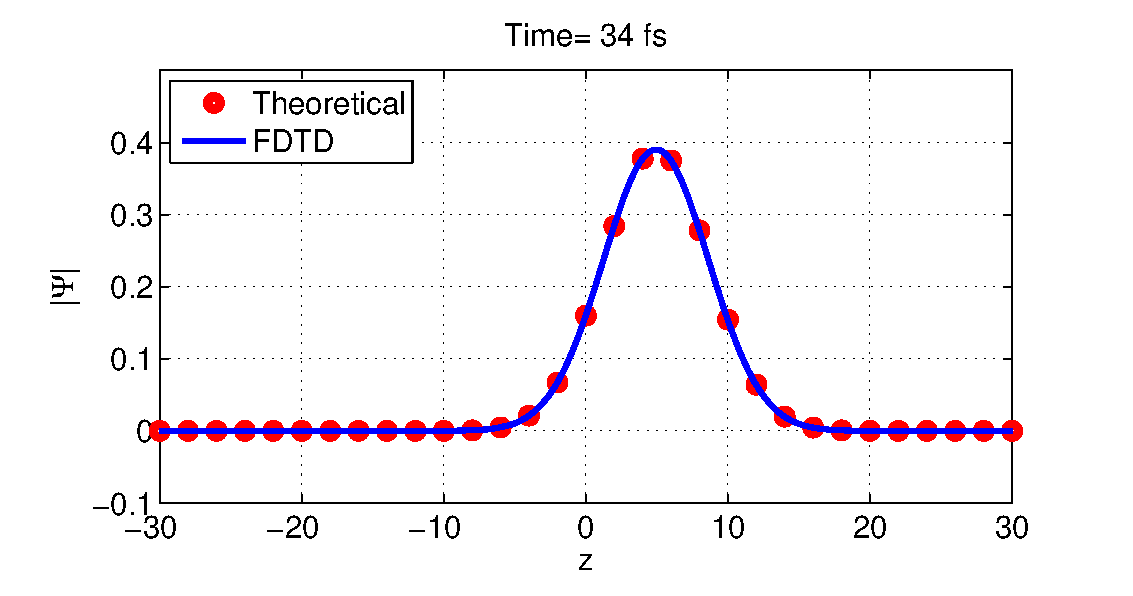
\includegraphics[scale=0.6]{34fs.eps}
\end{minipage}
\begin{minipage}[b]{1\linewidth}
\centering
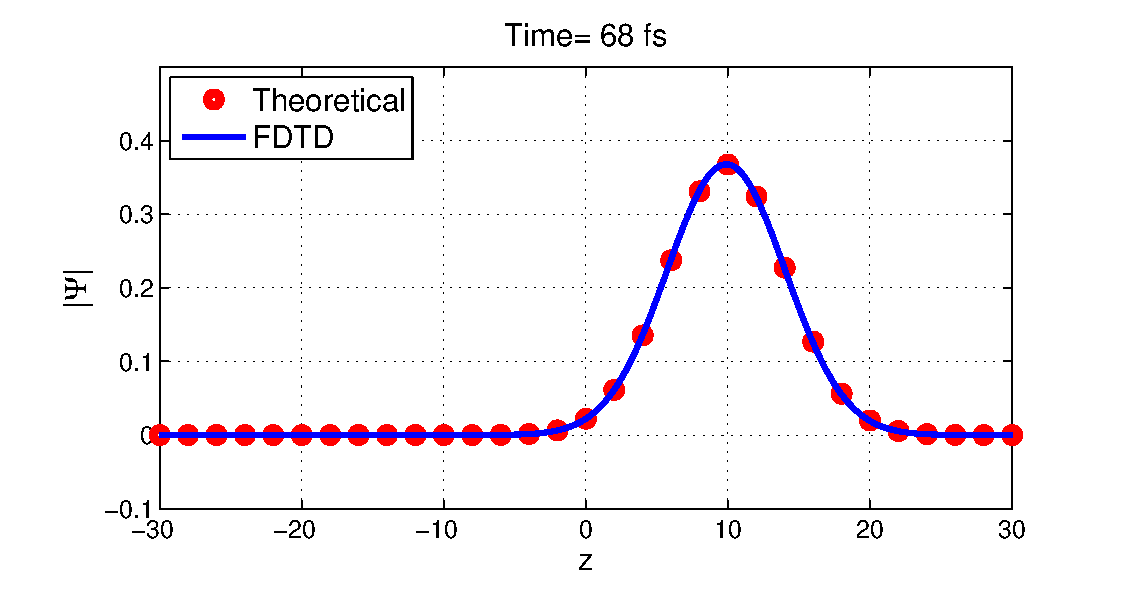
\includegraphics[scale=0.6]{68fs.eps}
\end{minipage}
\caption{\small  $\abs{\Psi(r,t)}$ for two time steps. The solid lines show our FDTD analysis and the the circles are the theoretical results obtained from \eqref{P5-integral}}
\label{fig:Psi}
\end{figure}

\newpage
Figure \ref{fig-new} has been also given to show the carrier frequency modulated by the Gaussian function obtained from FDTD simulation . $\abs{\Psi}^2$ at $t=34\mathrm{fs}$ and $t=68\mathrm{fs}$ have been shown  in the same figure. 

%----------New-------------
\begin{figure}[!h]
 \begin{minipage}[b]{0.5\linewidth}
 \centering
 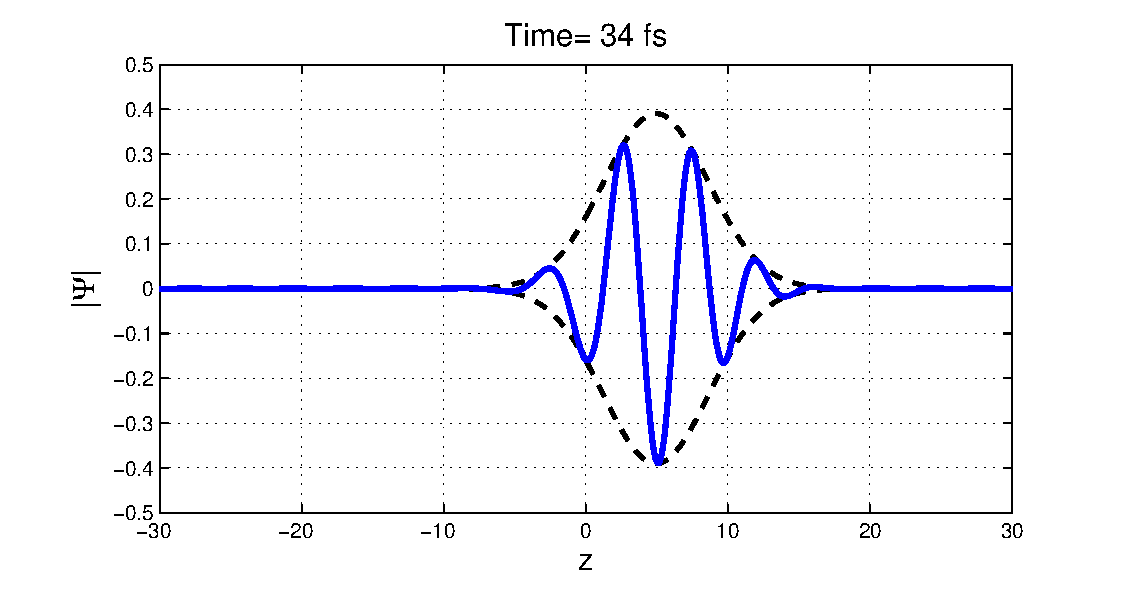
\includegraphics[scale=0.5]{psi_34.eps}
 \centerline{\small (a)}
  \end{minipage}
 \hspace{0.5cm}
 \begin{minipage}[b]{0.5\linewidth}
 \centering
 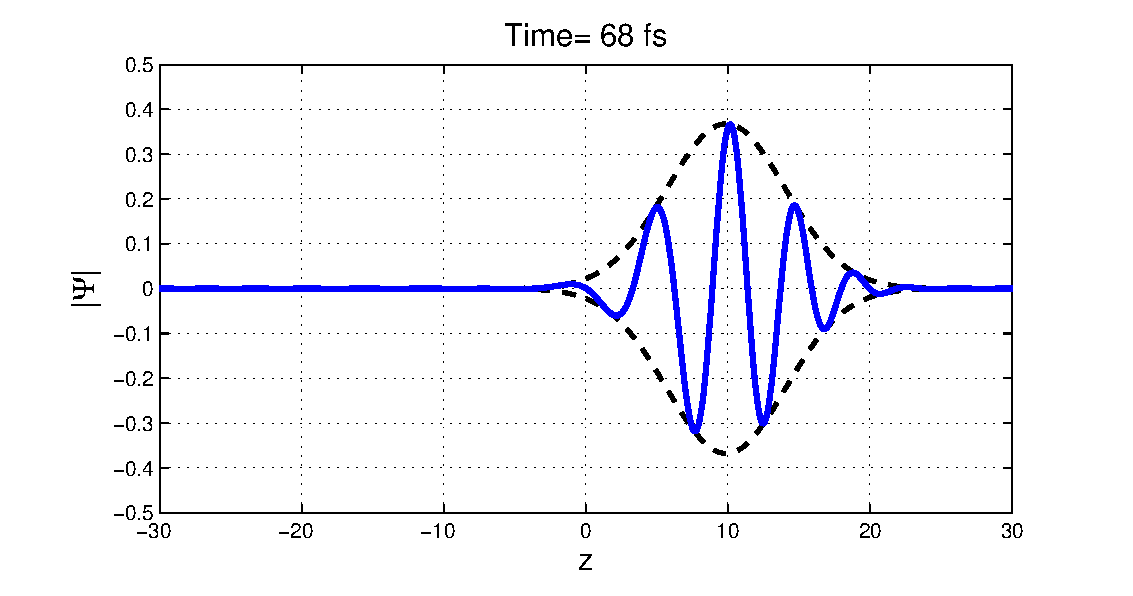
\includegraphics[scale=0.5]{psi_68.eps}
 \centerline{\small (c) }
 \end{minipage}
\begin{minipage}[b]{0.5\linewidth}
 \centering
 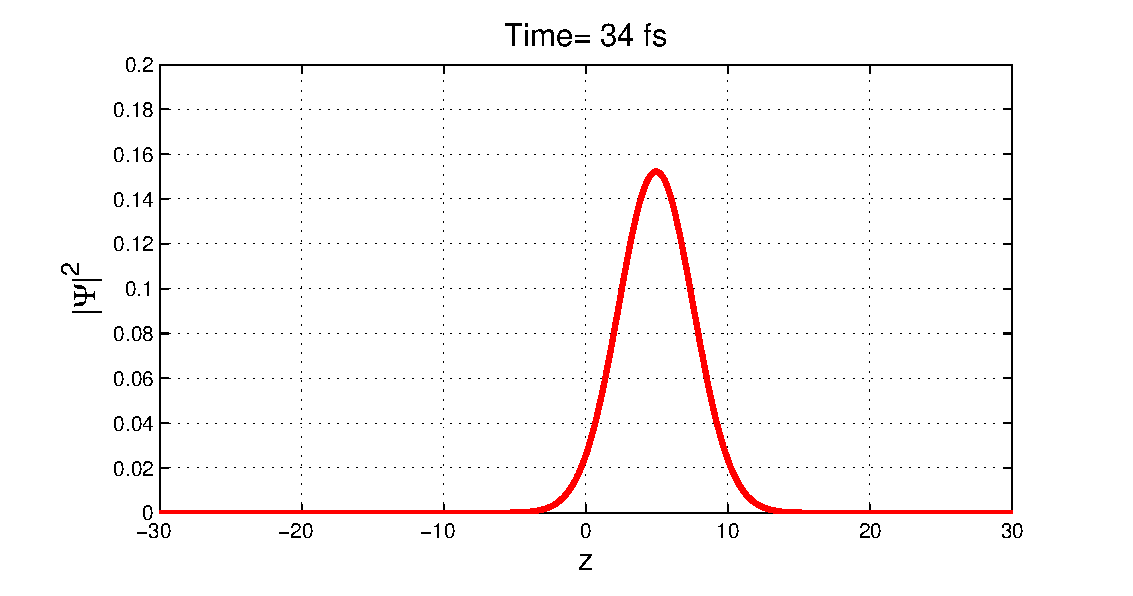
\includegraphics[scale=0.5]{pis2_34.eps}
 \centerline{\small (b)}
  \end{minipage}
  \hspace{0.5cm}
 \begin{minipage}[b]{0.5\linewidth}
 \centering
 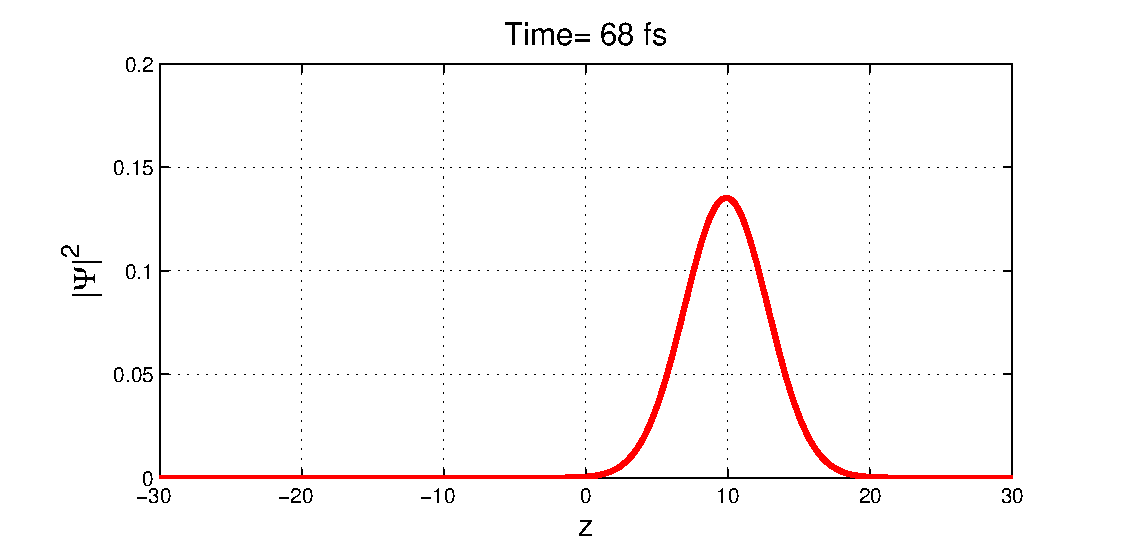
\includegraphics[scale=0.5]{psi2_68.eps}
 \centerline{\small (d)}
 \end{minipage}
  \caption{\small (a) the carrier frequency that is modulated by Gaussian at $t=34 \mathrm{fs}$ 
  (b) $\abs{\Psi(r,t)}^2$ at $t=34\mathrm{fs}$  
  (c) the carrier frequency that is modulated by Gaussian at $t=68 \mathrm{fs}$ 
  (d) $\abs{\Psi(r,t)}^2$ at $t=68\mathrm{fs}$  }
 \label{fig-new}
 \end{figure}
%---------------------------


\newpage
The normalization condition of the $\abs{\Psi}^2$ has to preserve in time. Total probability of finding the is plotted in figure \ref{fig:prob}. Obviously this quantity is preserved while the wave packet is inside the integration region. Please note that to clarify the details of the figure \textbf{total probability is plotted in $dB$ scale}. Maximum relative error is:
\begin{equation}
e_{\max}=\abs{P-1}_{\max}\times 100\%\approx 1.65\times 10^{-4}\%
\end{equation}  

\begin{figure}[!h]
\centering
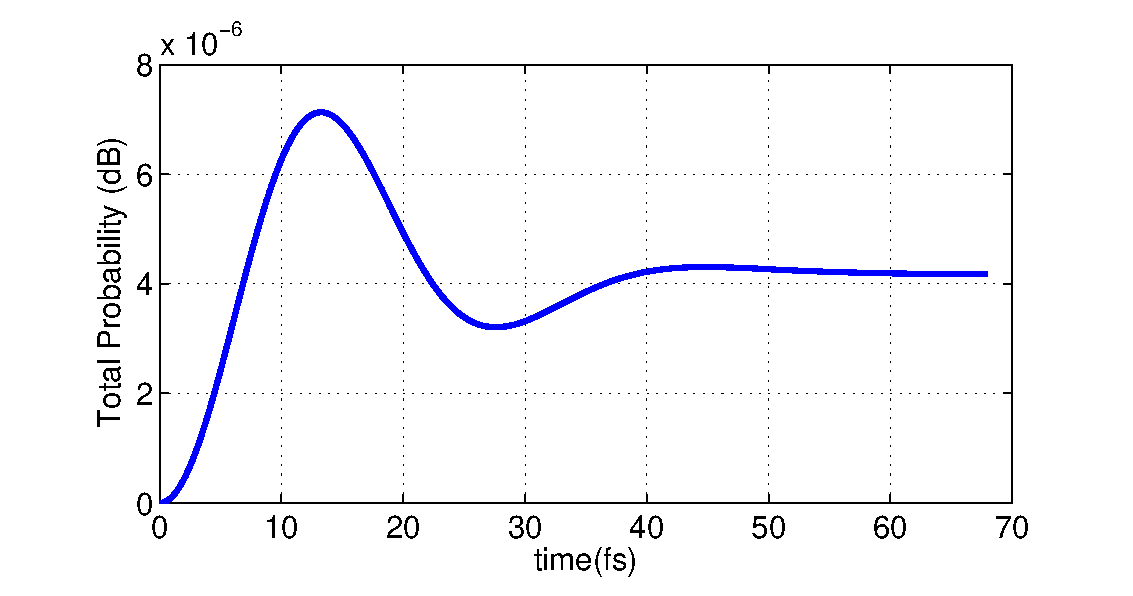
\includegraphics[scale=0.6]{probability.eps}
\caption{\small  Total probability in $dB$ scale versus time. The normalization condition of the $\abs{\Psi}^2$ is  preserved in time. }
\label{fig:prob}
\end{figure} 


The another quantity that should be preserved in time is the expectation value of the kinetic energy of the particle. As discussed in the previous section it's anticipated that the kinetic energy to be so close to the classical value calculated based on the group velocity of the wave packet. Hhowever there may be a small deviation which is purely quantum mechanical (since it's a quadric function of $\hbar$). Figure \ref{fig-KK} shows the expectation value of the kinetic energy (solid line)in time.
First, as it can be observed the kinetic energy is a constant of motion and very small fluctuations originate from the numerical errors. The classical prediction is also shown in the same figure (dash line). As it's anticipated from the equation \eqref{P5-Kclas} classical value of the kinetic energy is a bit smaller than the the expectation value in the real quantum state. The difference of these quantities is also plotted in figure \ref{fig:K-Kclassic}. Amazingly the difference agrees well with the equation \eqref{P5-Kclas}. Equation \eqref{P5-Kclas} predicts that the difference is:
$$\langle K\rangle-K_{classic}=\frac{\hbar^2}{2m\sigma^2}\approx 0.0015 \mathrm{ev}$$
All data on the vertical axis in figure \ref{fig:K-Kclassic} are in the same order of the predicted value.



%-----Figure-----------------------
\begin{figure}[!h]
\centering
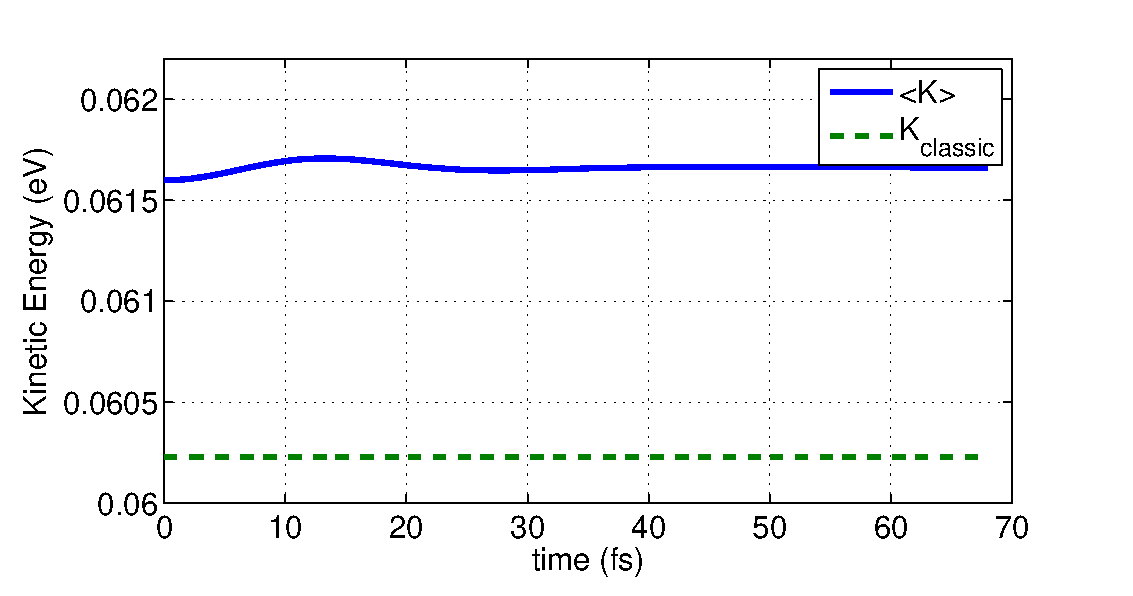
\includegraphics[scale=0.6]{K.eps}
\caption{\small  Expectation value of the kinetic energy (solid line) and classically expected value (dash-line). }
\label{fig-KK}
\end{figure} 
%-----Figure-------------------
\begin{figure}[!h]
\centering
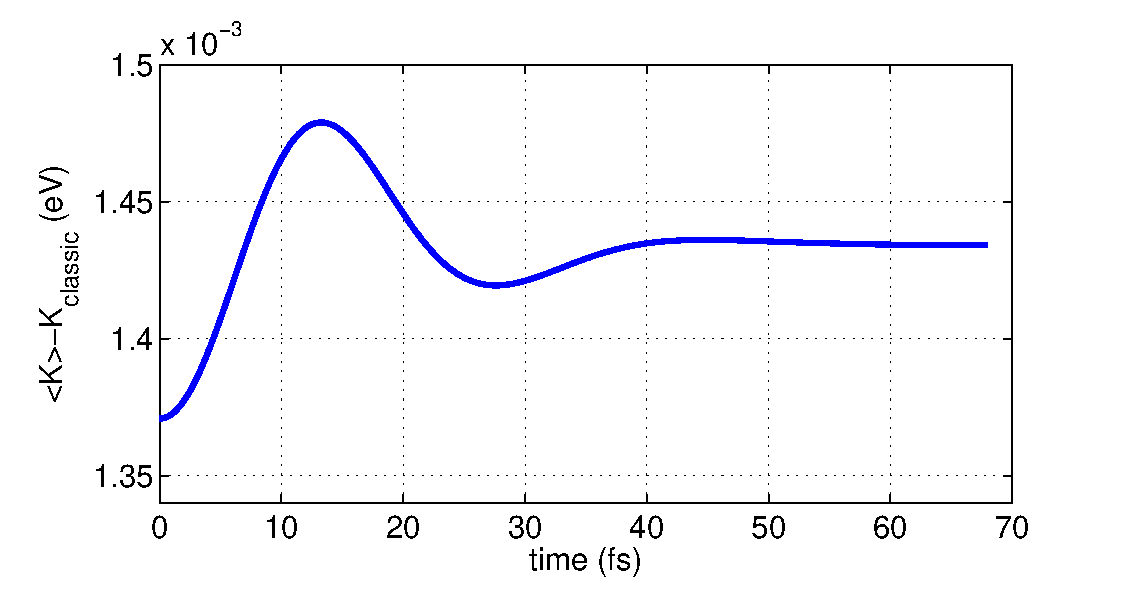
\includegraphics[scale=0.6]{K-Kclassic.eps}
\caption{\small  $\langle K\rangle -\frac{1}{2}mv_g^2$  }
\label{fig:K-Kclassic}
\end{figure} 

%-------------------------------




\end{homeworkSection}


\begin{homeworkSection}{Stability Analysis}
Time dicretization $\Delta t$ is time increment between consecutively calculated wave function in the numerical approach. The choice of $\Delta t$ is critical is the FDTD simulation. Undoubtedly, computation cost decreases as $\Delta t$ increases. However it is shown here that there is an upper bound for $\Delta t$ which ensures stability and prevents numerical error accumulation. As a matter of the fact, the time step should be chosen as a balance between computational cost and stability. Of course , the best time step would be the longer one so that the algorithm stability is maintained \cite{taflove}. 

The study of the numerical stability is analytically feasible through the eigenfunction decomposition technique. The wave function can be expressed as a continuous spectrum of the plane-wave functions satisfying Schr\"odinger equation. Our numerical scheme determines a specific growth factor the eigenfunction components. In the free space problem  plane wave propagating functions (eigenfunctions) are:


\begin{equation}
\T{\Psi}(k,t,z)=\exp\left(i\omega t-kz\right)
\end{equation}     

The discrete version of the Schr\"odinger's equation can be used to determine the \textit{growth factor} of each wave component. Actually the numerical discretization of the determines the time evolution of the wave components and naturally the eigenfunctions are numerically subject to a special temporal dependence. In this case the time evolution of the plane wave functions can be described by a growth factor ($q$). The growth factor is defined as :
\begin{equation}
q=\exp(j\T{\omega}\Delta t)=\frac{\T{\Psi}(k,(n+1)\Delta t,s\Delat z)}{\T{\Psi}(k,n\Delta t,s\Delat z)}
\end{equation} 
In above equation $\T{\omega}$ is a complex number which represents the numerical error accumulation in the discrete Schr\"odinger's equation. The numerical scheme is generally stable if and only if $\abs{q}\leq 1$ for all wave components. If we apply this theory to the couple equations \eqref{coupled1} and \eqref{coupled2} we get (for free particle):

\begin{align}
&\left(1-q^{-1}\right)\T{\Psi}_i(k,s,n+0.5) =2\xi\left[\cos(k\Delta z)-1\right]\T{\Psi}_r(k,s,n)\\
&\left(q-1\right)\T{\Psi}_r(k,s,n)=-2\xi\left[\cos(k\Delta z)-1\right]\T{\Psi}_i(k,s,n+0.5) 
\end{align}
 
 To have non-zero solution we should put the determinant of the coefficents to zero:
  \begin{equation}
  \det
  \begin{bmatrix}
  & 1-q^{-1} &  4\xi \sin^2\left(\frac{k\Delta z}{2}\right)\\
  &-4\xi \sin^2\left(\frac{k\Delta z}{2}\right) & q-1
  \end{bmatrix}
  =0\Lrw q^2-2\alpha q+1=0
  \end{equation}  
 
 wherein 
 $$\alpha=1-8\xi^2\sin^{4}\left(\frac{k\Delta z}{4}\right)$$
 
To satisfy the stability condition $\alpha$ should varies as:
\begin{equation}
\abs{q}\leq 1\Lrw\abs{\alpha}\leq 1\qquad \text{for all $k$}
\end{equation}
This constraint leads to the following bound for $\xi$:
\begin{equation}
\xi=\frac{\hbar\Delta t}{2m(\Delta x)^2}\leq \frac{1}{2}
\end{equation} 
To check the stability condition in our FDTD analysis we first define the energy of the wave function inside the integration region as:
\begin{equation}\label{P-def}
P=\int\abs{\Psi(z,t)}^2dz
\end{equation} 
This parameter can be used to show whether the algorithm is stable or not. In the figure \eqref{fig:stability} $P$ is plotted for four different values of $\xi$. Vertical axises show $P$ defined in \eqref{P-def} \textbf{in dB scale}. Obviously for $\xi=0.15$ and $\xi=0.5$ which are below the critical value ($0.5$) the algoithm is stable but for $\xi=0.51$ and $\xi=0.7$ FDTD analysis is conspecuously unstable and diverges.

\begin{figure}[t]
\begin{minipage}[b]{1\linewidth}
\centering
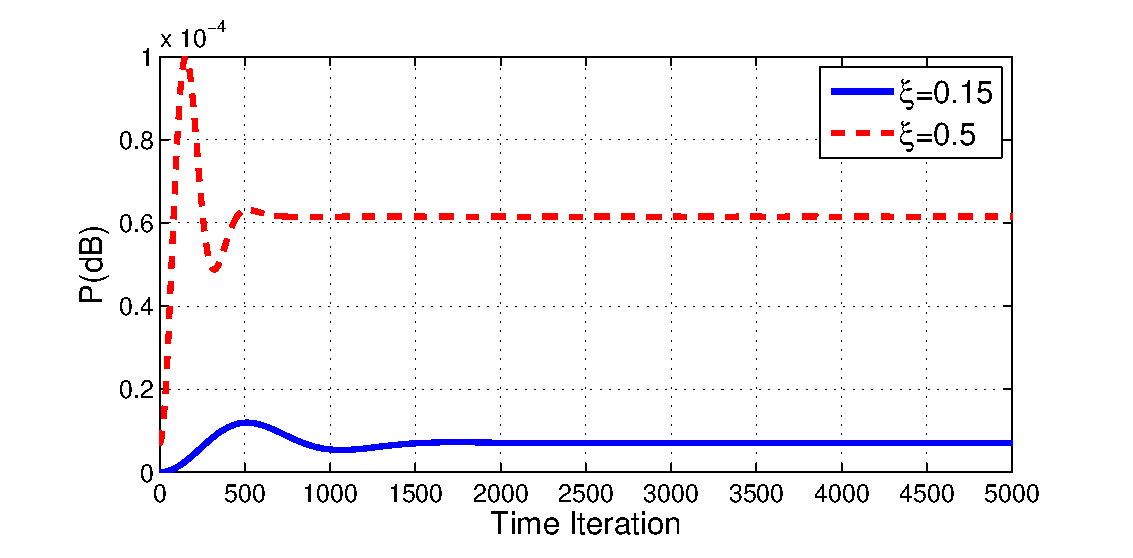
\includegraphics[scale=0.6]{stable.eps}
\centerline{\small (a) }
\end{minipage}
\begin{minipage}[b]{1\linewidth}
\centering
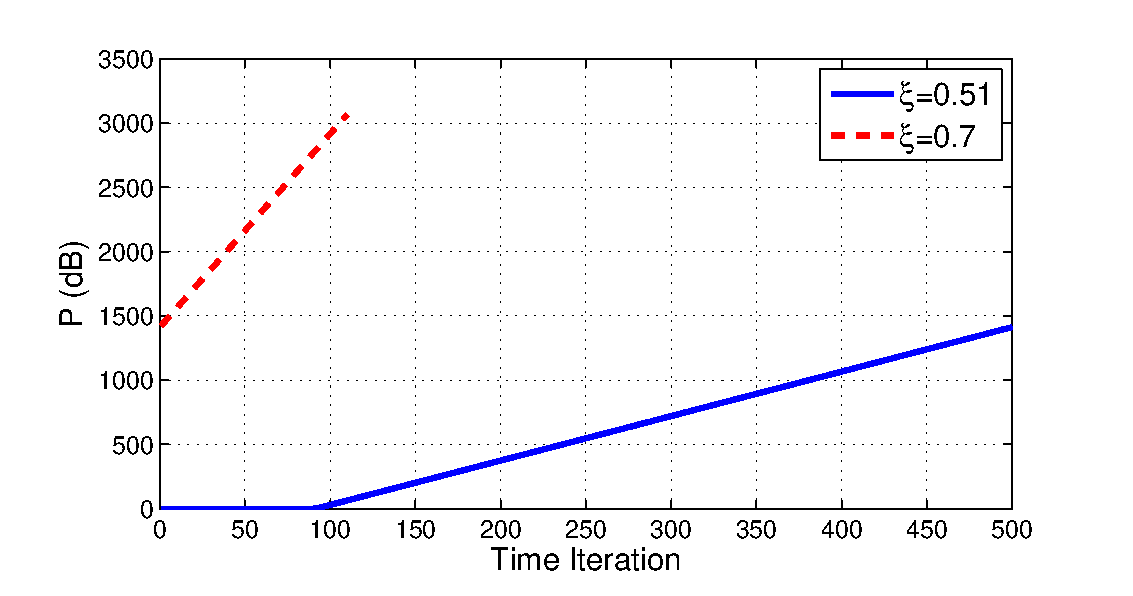
\includegraphics[scale=0.6]{unstable.eps}
\centerline{\small (b) }
\end{minipage}
\caption { \small  (a) Two stable FDTD simulations for $\xi=0.15$ and $\xi=0.5$. Both are smaller than the critical value. (b) Two unstable FDTD simulations for $\xi=0.51$ and $\xi=0.7$. Both don't satisfy stability condition} 
\label{fig:stability}
\end{figure}

\end{homeworkSection}

\begin{homeworkSection}{Absorbing Boundary Condition}

A number of techniques have been considered for boundary conditions which would remove spurious reflection from artificial boundaries during the numerical solution of the one-dimensional Schr\"odinger's equation. For example Kosloff and Kosloff \cite{kosloff} used an enlarged computational domain and then applied a damping in arificial part of the domain to decrease the amplitude of outgoing wave. Although this method can produce good results, the enlarged domain is costly, especially for extensions to higher dimensions. In this project we have implementted Shibata's absorbing boundary condition \cite{shibata}. This work is based primarily one the work of Enquist and Majd \cite{majd} which leads to one-way absorbing boundary conditions for the Schr\"odinger equation. From the basic principle of the quantum mechanics $k$ and $\omega$ satisfy the dispersion relation:
\begin{equation}\label{dispersion}
\hbar^2k^2=2m\left( \hbar\omega-V\right)
\end{equation}
Solving \eqref{dispersion} in terms of $\hbar k$, we get:
\begin{equation}\label{oneway}
\hbar k=\pm\sqrt{2m(\hbar\omega -V)}
\end{equation}

In this equation, plus and minus signs means the right going and left-going waves, respectively. Thus, the absorbing boundary conditions should be designed to satisfy the dispersion relation given by the plused-signed equation \eqref{oneway} at the boundary at right and the minus-signed equation \eqref{oneway} at the left boundary. These are the one-way equations   for the wave function. Unfortunately, function \eqref{oneway} is not rational and connot be converted into a partial differential equation. We can just make an approximation \cite{shibata}:
\begin{equation}\label{linear}
\hbar k\approx\pm\frac{\sqrt{2m\alpha_2}-\sqrt{2m\alpha_1}}{\alpha_2-\alpha_1}(\hbar\omega-V)
\pm\frac{\alpha_2\sqrt{2m\alpha_1}-\alpah_1\sqrt{2m\alpha_2}}{\alpha_2-\alpha_1}
\end{equation}  
where $\alpha_1$ and $\alpha_2$ are adjustable parameters. Equation \eqref{linear} is a straight line interpolation of equation \eqref{oneway}, which intersects the dispersion relations at two points. The correspondance of $\pds{t}\Leftrightarrow-i\omega$ and $\pds{z}\Leftrightarrow ik$ leads us to write this partial differential equation \cite{shibata}:
\begin{equation}\label{P5-main}
i\hbar\pd{\Psi(z,t)}{t}=\left[-i\hbar\frac{1}{g_1}\pds{z}-\frac{g_2}{g_1}\right]\Psi(z,t)
\end{equation}  
This equation has be written for free particle. In his equation $g_1$ and $g_2$ are \cite{shibata}:
\begin{align}
&g_1=\pm\frac{\sqrt{2m\alpha_2}-\sqrt{2m\alpha_1}}{\alpha_2-\alpha_1}\\
&g_2=\pm\frac{\alpha_2\sqrt{2m\alpha_1}-\alpah_1\sqrt{2m\alpha_2}}{\alpha_2-\alpha_1}
\end{align} 

Equation \eqref{P5-main} has been implemented in FDTD simulation and the result is plotted here. $\alpha_1=k^2_0\hbar^2/{m}$ and $\alpha_2 =5k_0^2\hbar^2/m$ are chosen for adjustable parameters.  

Figure \ref{fig:ABC} shows the wave reflection from the boundary. As we can see the wave absorption is not complete however it's acceptable for practical simulations. 


\begin{figure}[h]
\begin{minipage}[b]{1\linewidth}
\centering
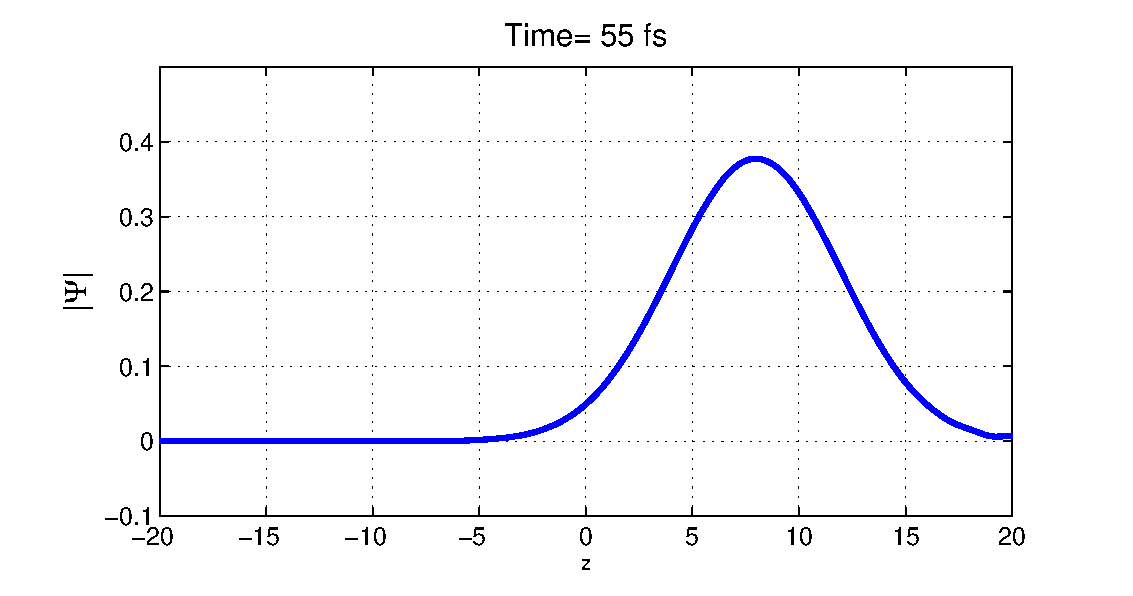
\includegraphics[scale=0.6]{ABC_before.eps}
\centerline{\small (a) }
\end{minipage}
\begin{minipage}[b]{1\linewidth}
\centering
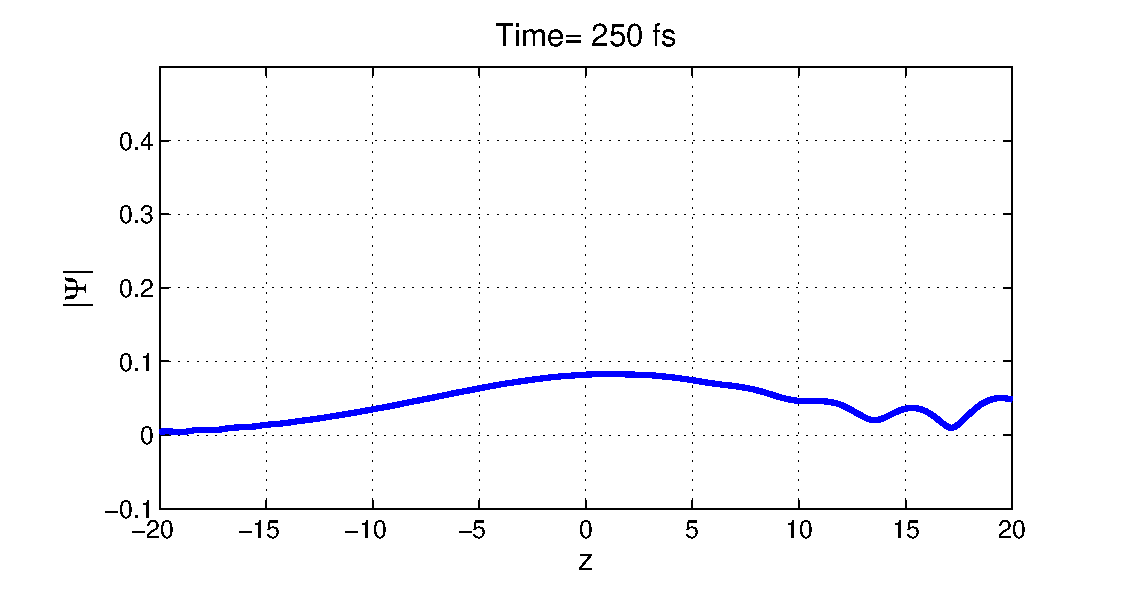
\includegraphics[scale=0.6]{ABC_after.eps}
\centerline{\small (b) }
\end{minipage}
\caption { \small $\abs{\Psi}$ (a) before the wave impinges to the boundary . (b)  after reflection} 
\label{fig:ABC}
\end{figure} 

Parameter $P$  defined in \eqref{P-def2} is also plotted in Figure \ref{fig:ABC_prob}. This parameter shows how much power reflects back to the region of integration.

\begin{equation}\label{P-def2}
P=\int_{z_l}^{z_r}\abs{\Psi}^2dz
\end{equation}

As it's shown in figure \ref{fig:ABC_prob} energy of the wave function is conspicuously reduced after reflection. This shows that the wave has been absorbed by the boundary.
%-----Figure-----------------------
\begin{figure}[!h]
\centering
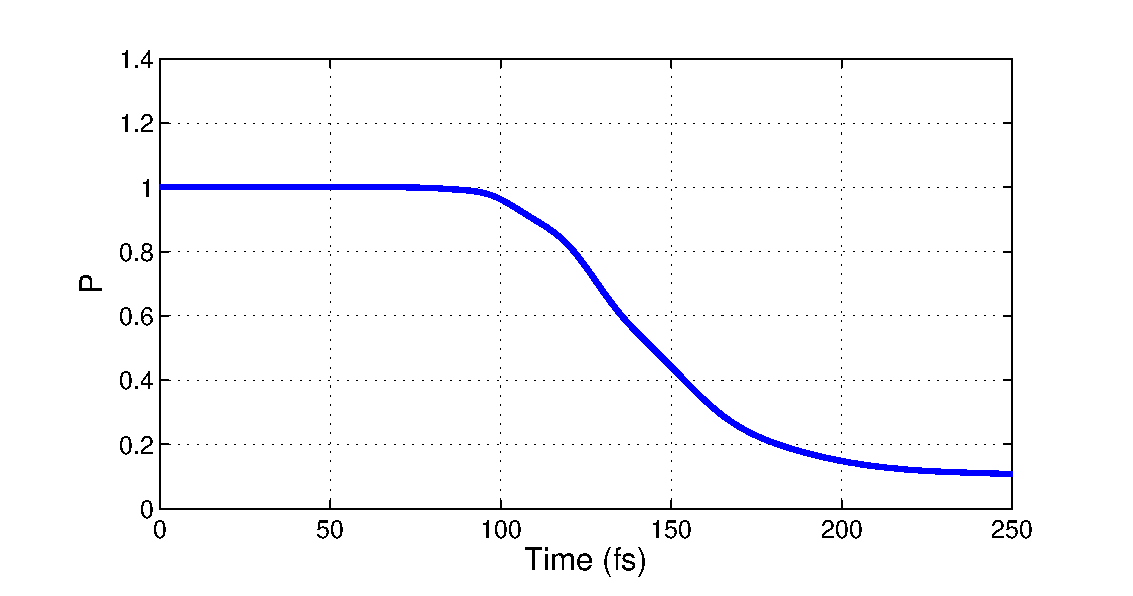
\includegraphics[scale=0.6]{ABC_prob.eps}
\caption{\small  Energy of the wave function inside the region. Total probability (energy) is constant befor impinging to the boundary and reduces after reflection }
\label{fig:ABC_prob}
\end{figure} 

%------------------------------------
\end{homeworkSection}
\end{homeworkProblem}